%label:"fig:polterovichSurgeryProfile"
%author:JeffHicks
%name:"surgery profile"
%type:"figure"
%parent:"def:polterovichSurgery"
%caption:"Surgery Profile for Polterovich surgery"



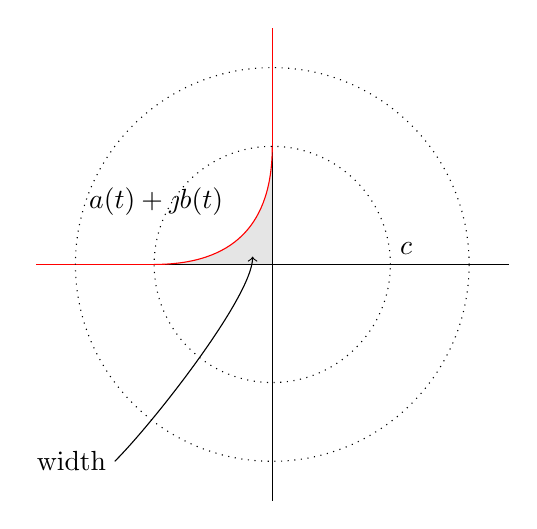
\begin{tikzpicture}

    \fill[fill=gray!20] (-1.5,0) .. controls (-0.5,0) and (-0.5,0) .. (0,0) .. controls (0,0.5) and (0,0.5) .. (0,1.5) .. controls (0,0.5) and (-0.5,0) .. (-1.5,0);
    
    \draw (0,3) -- (0,-3);
    \draw (3,0) -- (-3, 0);
    \draw[red] (-3, 0)--(-1.5,0) (0,1.5)--(0, 3);
    \draw[red] (-1.5,0) .. controls (-0.5,0) and (0,0.5) .. (0,1.5);
    \node[above left] at (-0.5,0.5) {$a(t)+\jmath b(t)$};
    \node[above right] at (1.5,0) {$c$};
    \draw[dotted]  (0,0) ellipse (1.5 and 1.5);
    \draw[dotted]  (0,0) ellipse (2.5 and 2.5);
    \draw[->] (-2,-2.5) .. controls (-1.5,-2) and (-0.25,-0.4) .. (-0.25,0.1);
    \node at (-2.55,-2.5) {width};
\end{tikzpicture}